\documentclass{beamer}

\usepackage{listings}
\usepackage{framed}
\usepackage{caption}
\usepackage{color}
\usepackage{xcolor}
\usepackage{amsfonts}
\lstset{
    language=C,
    frame=tb,
    %numbers=left,
    %stepnumber=1,
    %numbersep=5pt,
    backgroundcolor=\color{white},
    showspaces=false,
    showstringspaces=false,
    showtabs=false,
    tabsize=4,
    captionpos=b,
    breaklines=true,
    breakatwhitespace=true,
    keywordstyle=\color{blue},
    commentstyle=\color{magenta}\itshape,
    emphstyle=\color{red},
    stringstyle=\color{purple},
    identifierstyle=\color{cyan}
    %title=\lstname
}

\usetheme{Boadilla}

\title{Introduction to C Programming}
\author{Oliver Masters \\ \texttt{oliver.masters@ibm.com}}
\date{15th August 2018}

\begin{document}

\begin{frame}
\titlepage
\end{frame}

\section{Overview of the Language}

\begin{frame}
    \frametitle{What is C?}
    \begin{itemize}[<+->]
        \item General-purpose, imperative, procedural  programming language
        \item Compiled
        \item Extremely portable
        \item Static, weak typing 
        \item Higher level than assembly, but low-level memory access available
    \end{itemize}
\end{frame}

\begin{frame}
    \frametitle{Brief history of C}
    \begin{columns}
        \column{0.5\textwidth}

        \begin{itemize}[<+->]
            \item First released 1972
            \item AT\&T
            \item Developed alongside Unix by K\&R
            \item 5 standards in total, latest: C11
            \item Influenced almost every major language since
        \end{itemize}

        \column{0.25\textwidth}

        \begin{figure}
            \centering
            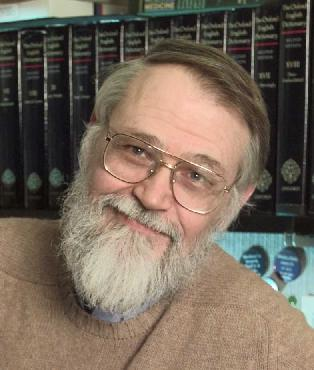
\includegraphics[width=\textwidth]{briankernighan.jpg}
            \caption*{Brian Kernighan}
            \label{fig:kern}
        \end{figure}

        \column{0.25\textwidth}

        \begin{figure}
            \centering
            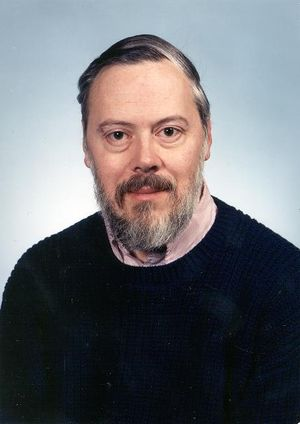
\includegraphics[scale=0.5]{dennisritchie.jpg}
            \caption*{Dennis Ritchie}
            \label{fig:ritch}
        \end{figure}
    \end{columns}
\end{frame}

\begin{frame}
    \frametitle{Why learn or use C?}
    \begin{itemize}[<+->]
        \item Extremely fast to execute
        \item Unbeatable portability
        \item Very mature -- systems critical to safety
        \item Microcontrollers/embedded systems
        \item Kernel and driver development
        \item Deeper understanding of algorithms and data structures
    \end{itemize}
\end{frame}

\section{Technical Details}

\begin{frame}
    \frametitle{Hello World}
    \begin{figure}
        \lstinputlisting{../Code/HelloWorld/hello.c}
    \end{figure}
\end{frame}

\end{document}
